\documentclass{article}
\usepackage[margin = 1in]{geometry}
\usepackage{tcolorbox}
\usepackage{enumerate}
\usepackage{ragged2e}
\usepackage{amsmath}
\usepackage{amssymb}
\usepackage{fancyhdr}
\usepackage{booktabs}
\usepackage{subfig}
\usepackage{epstopdf}
\usepackage{xcolor}
\usepackage{dsfont}
\usepackage[justification=centering]{caption}

\renewcommand{\vec}[1]{\mathbf{#1}}
\newcommand{\qed}{\hfill$\blacksquare$}
\newcommand{\var}{\mathrm{Var}}
\newcommand{\abs}[1]{\left\lvert{#1}\right\rvert}
\newcommand{\norm}[1]{\left\lvert\!\lvert{#1}\right\rvert\!\rvert}

\begin{document}

\RaggedRight
\pagestyle{fancy}

\rhead{\footnotesize\uppercase{16-831: Statistical Techniques in Robotics}} 

{\large Project 3: List Prediction and Online SVM} \\[0.5\parsep]
Dawei Wang (daweiwan@andrew.cmu.edu)

\vspace{1em}
{\large\bf Theoritical: List Prediction}

\begin{itemize}

	\item 1.2.1: Monotone Submodularity: 
	
		{\bf\small MONOTONICITY}: $\forall L_1,L_2,T\subseteq S$, 
		$L_1\cap T\subseteq(L_1\cup L_2)\cap T$, \footnote{$\forall x\in L_1\cap T$,
			$x\in L_1$ and $x\in T$; therefore $x\in L_1\cap L_2$, and $x\in(L_1\cup L_2)\cap T$.}
 		$\Rightarrow\abs{L_1\cap T}\le\abs{(L_1\cup L_2)\cap T}$, therefore
 		$f(L_1;T)=\min(1,\abs{L_1\cap T})\le\min(1,\abs{(L_1\cup L_2)\cap T})=f(L_1\cup L_2;T)$;
 		
 		{\bf\small SUBMODULARITY}: $\forall L_1,L_2,T\subseteq S$, and $\forall s\in S$, we have	
 		\begin{flalign}
 			b(s|L_1)&=f(L_1\cup\{s\};T)-f(L_1;T)\label{bs1}\\
 			b(s|L_1\cup L_2)&=f(L_1\cup L_2\cup\{s\};T)-f(L_1\cup L_2;T)\label{bs2}
 		\end{flalign}
 		consider the following cases:
 		\begin{itemize}
 			\item $s\in L_1\Rightarrow L_1\cup\{s\}=L_1,L_1\cup L_2\cup\{s\}=L_1\cup L_2
 				\Rightarrow b(s|L_1)=0\ge0=b(s|L_1\cup L_2)$; 
			\item $s\not\in L_1$, $s\in L_2\Rightarrow L_1\cup L_2\cup\{s\}=L_1\cup L_2$
				$\Rightarrow b(s|L_1)\ge0$ (monotonicity) $=b(s|L_1\cup L_2)$; 
			\item $s\not\in L_1$, $s\not\in L_2$, $s\in T$, 
				from Equations (\ref{bs1}) and (\ref{bs2}): 
			\begin{flalign}
				b(s|L_1)&=\min(1,\abs{(L_1\cup\{s\})\cap T})-f(L_1;T)\\
					&=\min(1,\abs{(L_1\cap T)\cup(\{s\}\cap T)})-f(L_1;T)\label{bs1t}\\
					&=\min(1,\abs{L_1\cap T}+1)-f(L_1;T)=1-f(L_1;T)\\
				b(s|L_1\cup L_2)&=\min(1,\abs{(L_1\cap L_2\cap T)\cup(\{s\}\cap T)})-
					f(L_1\cup L_2;T)\label{bs2t}\\
					&=\min(1,\abs{L_1\cap L_2\cap T}+1)-f(L_1\cup L_2;T)=1-f(L_1\cup L_2;T)
			\end{flalign}
			since $f(L_1;T)\le f(L_2\cup L_2;T)$ (monotonicity), we have
				$b(s|L_1)\ge b(s|L_1\cup L_2)$; 
			\item $s\not\in L_1$, $s\not\in L_2$, $s\not\in T\Rightarrow \{s\}\cap T=\varnothing$,
				from Equations (\ref{bs1t}) and (\ref{bs2t}): 
				\begin{flalign}
					b(s|L_1)&=\min(1,\abs{L_1\cap T})-f(L_1;T)=0\\
					b(s|L_1,L_2)&=\min(1,\abs{L_1\cap L_2\cap T})-f(L_1\cup L_2;T)=0
				\end{flalign}
				we still have $b(s|L_1)=0\ge 0=b(s|L_1\cup L_2)$. 
 		\end{itemize}
 		therefore, the \emph{multiple guess} function is monotone and submodular. \qed
 		
 	\item 1.2.2: Greedy Guarantee: 
 			\begin{flalign}
			 {\bf\small STEP 1}:
 				\Delta_i&=f(L^*)-f(L_{i-1}^G)
 				\le f(L_{i-1}^G\oplus L^*)-f(L_{i-1}^G)\quad\text{(monotonicity)}\\
 				&=\textstyle\sum_{j=1}^k\left[f(L_{i-1}^G\oplus L_j^*)-f(L_{i-1}^G
 					\oplus L_{j-1}^*)\right]\\
 				&=\textstyle\sum_{j=1}^k\left[f(L_{i-1}^G\oplus L_{j-1}^*\oplus l_j^*)
 					-f(L_{i-1}^G\oplus L_{j-1}^*)\right]\\
 				&\le \textstyle\sum_{j=1}^k\left[f(L_{i-1}^G\oplus l_j^*)-f(L_{i-1}^G)\right]
 				\quad\text{(submodularity)}\\
 			{\bf\small STEP 2}: \Delta_i&
 				\le \textstyle\sum_{j=1}^k\left[f(L_{i-1}^G\oplus l_j^*)-f(L_{i-1}^G)\right]
 				\\ &\le\textstyle\sum_{j=1}^k\left[f(L_{i-1}^G\oplus l_i^G)-f(L_{i-1}^G)\right]
 				\quad\text{(greediness)}\\
 				&=\textstyle\sum_{j=1}^k\left[f(L_i^G)-f(L^*)\right]+\left[f(L^*)-f(L_{i-1}^G)\right]
 				\\&=\textstyle\sum_{j=1}^k\left[-\Delta_{i+1}+
 					\Delta_i\right]=k(\Delta_i-\Delta_{i+1})\\
 				\Delta_{i+1}&\le\left(1-1/k\right)\Delta_i\\
 			{\bf\small STEP 3}:\Delta_{k+1}&\le(1-1/k)\Delta_k\le(1-1/k)^k\Delta_1\le(1/e)\Delta_1\\
 				f(L^*)-f(L_G)&\le(1/e)f(L^*)\\
 				f(L_G)&\ge(1-1/e)f(L^*)
 			\end{flalign}
 			therefore, the greedy optimization policy ensures near-optimal performance. \qed
 		
\end{itemize}

\vspace{1em}
{\large\bf Theoritical: Online SVM}

\begin{itemize}
	\item 2.2.1: Formulation Equivalency: the constraints can be re-written as
	\begin{equation}
		\begin{split}
			\xi_i&\ge0\\
			\xi_i&\ge1-y_iw^Tf_i
		\end{split}
		\quad\Leftrightarrow\quad
		\xi_i\ge\max\left(0,1-y_iw^Tf_i\right)
	\end{equation}
	and the optimization can be performed sequentially with respect to $\xi$ and $w$:
	\begin{equation}
		\min_{\xi,w}\left[\frac{\lambda}{2}\norm{w}^2+\sum_{i=1}^T\xi_i\right]
		=\min_{w}\left[\frac{\lambda}2\norm{w}^2+\min_{\xi}\sum_{i=1}^T\xi_i\right]
		=\min_{w}\left[\frac{\lambda}2\norm{w}^2+\sum_{i=1}^T\max(0,1-y_iw^Tf_i)\right]
	\end{equation}
	therefore the two problem formulations are equivalent. \qed
	
	\item 2.2.2: Convexity: considering the objective function 
	\begin{equation}
		J(w;\mathcal{D})=\sum_{i=1}^T\left[\frac{\lambda}{2T}\norm{w}^2+\max(0,1-y_iw^Tf_i)\right]
	\end{equation}
	with $\forall w_1,w_2$ and $\gamma\in[0,1]$, we have
	\footnote{$\max(0,x+y)\le\max(0,x)+\max(0,y)$, since if $x+y\le0$, $\max(0,x+y)=0
		\le\max(0,x)+\max(0,y)$; otherwise, if $x+y>0$, $\max(0,x)+\max(0,y)\ge x+y=
		\max(0,x+y)$. Hence this inequality always holds regardless of $x$ and $y$. }
	\begin{flalign}
		\max(0,1-y_i[(1-\gamma)w_1+\gamma w_2]^Tf_i)&=\max(0, 
			(1-\gamma)(1-y_iw_1^Tf_i)+\gamma(1-y_iw_2^Tf_i))\\
			&\le\max(0,(1-\gamma)(1-y_iw_1^Tf_i))+\max(0,\gamma(1-y_iw_2^Tf_i))\\
			&=(1-\gamma)\max(0, 1-y_iw_1^Tf_i)+\gamma\max(0,1-y_iw_2^Tf_i)\\
		\norm{(1-\gamma)w_1+\gamma w_2}^2&\le
			(1-\gamma)^2\norm{w_1}^2+\gamma^2\norm{w_2}^2\quad\text{(triangle inequality)}\\
			&\le(1-\gamma)\norm{w_1}^2+\gamma\norm{w_2}^2
	\end{flalign}
	and combining both terms yields 
	\begin{flalign}
		J\left[(1-\gamma)w_1+\gamma w_2;\mathcal{D}\right]&\le\textstyle\sum_{i=1}^T
		\left[\frac{\lambda}{2T}\norm{(1-\gamma)w_1+\gamma w_2}^2+
			\max(0,1-y_i[(1-\gamma)w_1+\gamma w_2]^Tf_i)\right]\\
		&\le\textstyle\sum_{i=1}^T\frac{\lambda}{2T}
			((1-\gamma)\norm{w_1}^2+\gamma\norm{w_2}^2)\nonumber\\
			&\quad\quad+(1-\gamma)\max(0, 1-y_iw_1^Tf_i)+\gamma\max(0,1-y_iw_2^Tf_i)\\
		&=(1-\gamma)J(w_1;\mathcal{D})+\gamma J(w_2;\mathcal{D})
	\end{flalign}
	therefore this objective function is a convex function. \qed
	\item 2.2.3: Sub-gradient Descent: for $\forall w,u$, if $1-y_tw^Tf_t>0$
	\begin{flalign}
		l(w)+\nabla l_t(w)^T(u-w)&=l(w)+(\tfrac{\lambda}Tw^T-y_tf_t^T)(u-w)\\
		&=\tfrac{\lambda}{2T}\norm{w}^2+(1-y_tw^Tf_i)+\tfrac{\lambda}{T}w^Tu-y_tf_t^Tu
			-\tfrac{\lambda}{T}\norm{w}^2+y_tf_t^Tw\\
		&=-\tfrac{\lambda}{2T}\norm{w}^2+\tfrac{2\lambda}{2T}w^Tu+(1-y_tf_t^Tu)\\
		&=-\tfrac{\lambda}{2T}\norm{w-u}^2+\tfrac{\lambda}{2T}\norm{u}^2+(1-y_tf_t^Tu)\\
		&\le\tfrac{\lambda}{2T}\norm{u}^2+\max(0,1-y_tf_t^Tu)=l(u)
	\end{flalign}
	otherwise, i.e., if $1-y_tw^Tf_t\le0$, $\max(0,1-y_tw^Tf_t)=0$, we have
	\begin{flalign}
		l(w)+\nabla l_t(w)^T(u-w)&=l(w)+(\tfrac{\lambda}Tw^T)(u-w)\\
		&=\tfrac{\lambda}{2T}\norm{w}^2-\tfrac{\lambda}{T}\norm{w}^2+
		\tfrac{2\lambda}{2T}w^Tu\\
		&=-\tfrac{\lambda}{2T}\norm{w-u}^2+\tfrac{\lambda}{2T}\norm{u}^2+0\\
		&\le\tfrac{\lambda}{2T}\norm{u}^2+\max(0,1-y_tf_t^Tu)=l(u)
	\end{flalign}
	therefore the proposed sub-gradient $\nabla l_t(w)$ is valid. \qed
\end{itemize}


\newpage
{\large\bf Programming: List Prediction}\\[1em]

Run {\tt gen\_plots.m} to obtain Figure \ref{listpred}. A linear regressor is used
over all three algorithms for fair comparison; an extra intercept term is explicitly
appended to each feature vector (trajectory). It is expected that the success ratio
will be monotonically increasing as $k$ continues to grow; for both training and testing, 
list prediction strategies, with or without feature update, outperform the naive strategy
consistently. This can be explained by the fact that list prediction attempts to 
explore diverse options by greedily selecting the features that yield the greatest
marginal benefits, as opposed to the naive strategy which does not. This property
is particularly important when the benefit function is \emph{multiple guess}. Updating
the features essentially incorporates the diversity information into the features, allowing
the learner to exploit them more directly, therefore resulting in better accuracies. Testing
accuracies are generally lower than training accuracies due to generalization errors. \qed
\\[1em]

\begin{figure}
	\centering
	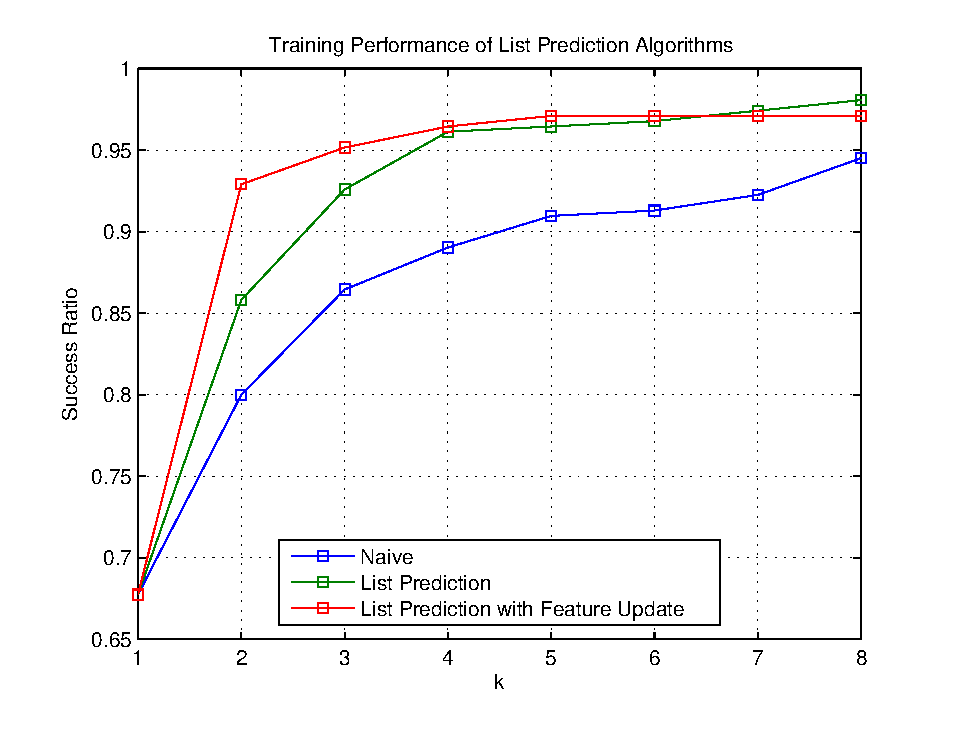
\includegraphics[width = 0.45\textwidth]{train.eps}
	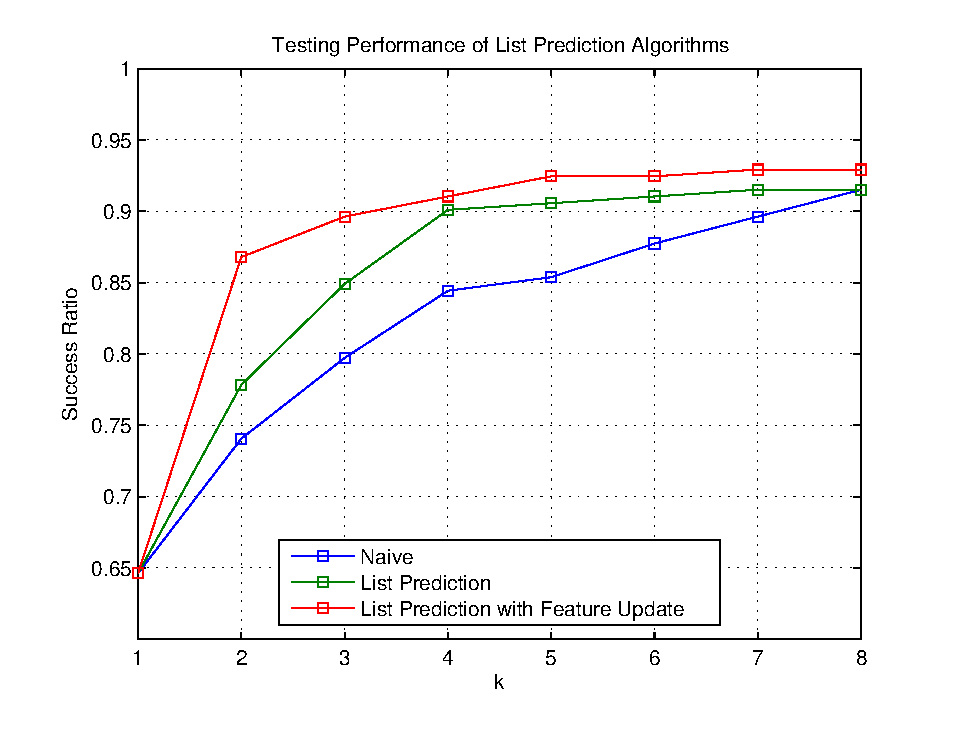
\includegraphics[width = 0.45\textwidth]{test.eps}	
	\caption{Performance of List Prediction Algorithms (Training: Left; Testing: Right)}
	\label{listpred}
\end{figure}

{\large\bf Programming: Online SVM}\\[1em]

Run {\tt gen\_results.m} to obtain Table \ref{onlinesvm}. (1) Each element dictates the binary
mis-classification error (chance error) when the online support vector machine is run on 
the dataset constructed by combining the data points from the two classes, as displayed
at its corresponding row and column titles. (2) Apparently there are a few combinations
that were not classified well (errors were marginally smaller than the chance errors)
such as (Pole, Vegetation), (Wire, Vegetation), (Pole, Facade), and (Wire, Facade). This
may be primarily attributed to the quality (distinctiveness) of the features. (3) It took
roughly 10 seconds to compute that table. The time complexity is linear in the number of
data points and the number of features. (4) The next page includes some images from 
select combinations of classes. \qed 

\begin{table}
	\centering
	\caption{Binary Mis-classification Errors (Chance Errors) (\%)} 
	\begin{tabular}{cccccc}\toprule
		&Vegetation&Wire&Pole&Ground&Facade\\ \midrule
		Count & 8322 & 818 & 1429 & 67161 & 12092 \\ \midrule
		Vegetation & - & 8.96 (8.95) & 11.08 (14.65) & 0.56 (11.02) & 16.56 (40.77)\\
		Wire & 8.96 (8.95) & - & 5.61 (36.40) & 0.20 (1.20) & 6.34 (6.34) \\
		Pole & 13.68 (14.65) & 6.19 (36.40) & - & 0.18 (2.08) & 10.13 (10.57) \\
		Ground & 0.55 (11.02) & 0.21 (1.20) & 0.19 (2.08) & - & 0.55 (15.26) \\
		Facade & 16.59 (40.77) & 6.34 (6.34) & 10.26 (10.57) & 0.53 (15.26) & - \\ \bottomrule
	\end{tabular}
	\label{onlinesvm}
\end{table}

\newpage
\begin{figure}
	\centering
	\subfloat[Ground vs. Vegetation]{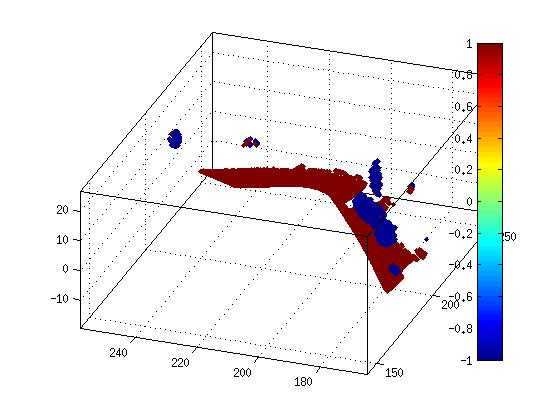
\includegraphics[width = 0.45\textwidth]{images/4vs1.jpg}}
	\subfloat[Ground vs. Wire]{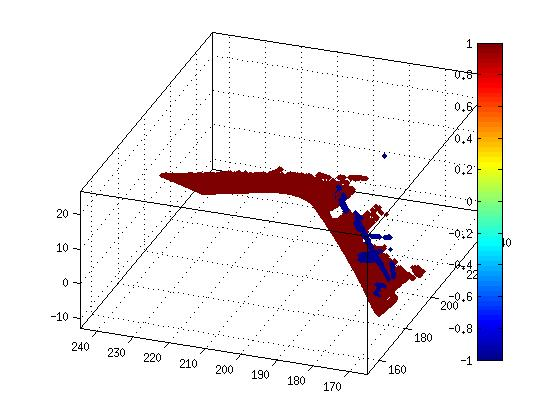
\includegraphics[width = 0.45\textwidth]{images/4vs2.jpg}} \\
	\subfloat[Ground vs. Pole]{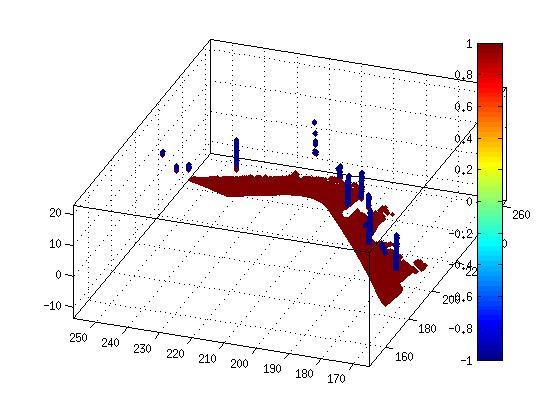
\includegraphics[width = 0.45\textwidth]{images/4vs3.jpg}}
	\subfloat[Ground vs. Facade]{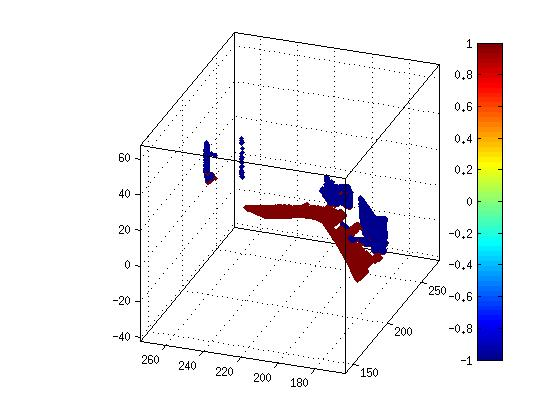
\includegraphics[width = 0.45\textwidth]{images/4vs5.jpg}}	
	\caption{Images of the Classified Data}
\end{figure}

{\large\bf Appendix: List of Functions and Scripts}\\[1em]
The implementation is entirely in MATLAB. 
\begin{itemize}\itemsep-1pt
	\item {\tt ftupdate.m}: update the features by appending similarity metrics;
	\item {\tt lblupdate.m}: update the labels by replacing them with marginal benefits;
	\item {\tt train.m}: train a linear regressor given features and labels;
	\item {\tt predict.m}: pick the best data point for each environment, given the model and features;
	\item {\tt naive.m}: the function that implements the naive prediction strategy;
	\item {\tt listpred.m}: the function that implements the list prediction strategy; 
	\item {\tt lpwftupdate.m}: the function that implements the list prediction strategy
		with feature update. 
	\item {\tt onlinesvm.m}: the function that implements online SVM; 
	\item {\tt gen\_plots.m}: a script that executes all the list prediction strategies;
	\item {\tt gen\_results.m}: a script that runs the online SVM on all possible pairs of classes; 
	\item {\tt fscatter3.m}: a third-party script that plots 3D point cloud in MATLAB; 
	\item {\tt data/}: a directory that contains all the data files. 
\end{itemize}
The submission also includes this writeup. 
		
\end{document}















